\subsection{Равномерное скрещивание}\label{SetOfOperatorsAlgorithms:UniformCrossover}

Идентификатор: \textbf{UniformCrossover}.

Данный оператор скрещивания используется для бинарных векторов.

Пусть имеется два родителя (родительские хромосомы) $\overline{Parent}^1$ и $\overline{Parent}^2$. Потомок состоит из генов, каждый из которых выбран случайно из генов родителей на соответствующих позициях. То есть скрещивание происходит по формулам:

\begin{align}
\label{SetOfOperatorsAlgorithms:eq:UniformCrossover}
&Crossover \left( \overline{Parent}^1, \overline{Parent}^2, DataOfCros\right) = \overline{Offspring};\\
& \overline{Offspring}_i=Random\left( \left\lbrace \overline{Parent}^1_i;\overline{Parent}^2_i\right\rbrace \right), i=\overline{1,n} ;\nonumber\\
&\overline{Offspring}\in X.\nonumber
\end{align}

\textbf{Пример.} Равномерное скрещивание показано на рисунке:

\begin{figure} [H]
  \center
  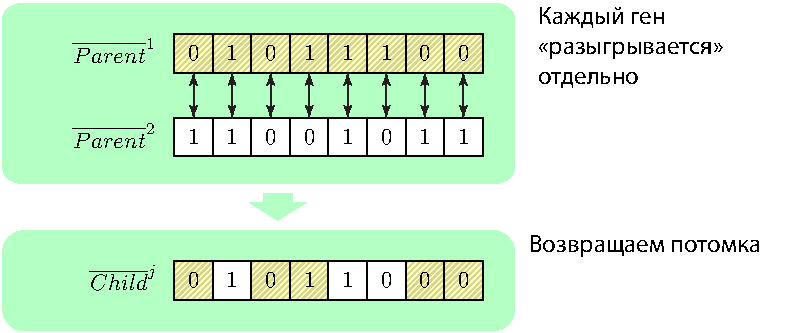
\includegraphics [scale=0.7] {UniformCrossover}
  \caption{Механизм работы равномерного скрещивания} 
  \label{SetOfOperatorsAlgorithms:img:UniformCrossover}  
\end{figure}

$ DataOfCros $ не содержит каких-либо параметров относительно данного типа скрещивания.

В библиотеке \textbf{HarrixMathLibrary} данная селекция реализуется через функцию \textbf{THML\_UniformCrossover}:

\href{https://github.com/Harrix/HarrixMathLibrary}{https://github.com/Harrix/HarrixMathLibrary}